\documentclass[a4paper,12pt]{article}

\usepackage[utf8]{inputenc}
\usepackage[english]{babel} 
\usepackage{graphicx}
\usepackage{geometry}
\usepackage{listings}
\usepackage{xcolor}
\usepackage{tikz}
\usetikzlibrary{shapes, arrows, positioning}

\geometry{top=2cm, bottom=2cm, left=2.5cm, right=2.5cm}
\definecolor{codegreen}{rgb}{0,0.6,0}
\lstdefinestyle{mystyle}{
    backgroundcolor=\color{white},   
    commentstyle=\color{codegreen},
    keywordstyle=\color{blue},
    basicstyle=\ttfamily\footnotesize,
    breakatwhitespace=false,         
    breaklines=true,                 
    captionpos=b,                    
    keepspaces=true,                 
    numbers=left,                    
    numbersep=5pt,                  
    showspaces=false,                
    showstringspaces=false,
    showtabs=false,                  
    tabsize=2,
    frame=single
}
\lstset{style=mystyle}
\title{\textbf{Practical Work 5: The Longest Path using MapReduce}}
\author{Group Name: ...}
\date{\today}

\begin{document}

\maketitle

\section{Introduction}
The objective of this practical work is to implement a system to find the longest file path within a dataset using the \textbf{MapReduce} programming model. The input data consists of a list of file paths generated by the system command \texttt{find}.

\section{MapReduce Design}

\subsection{Algorithm}
\begin{itemize}
    \item \textbf{Input Split:} The large input file is divided into smaller chunks to be processed in parallel.
    \item \textbf{Mapper:} 
        \begin{itemize}
            \item \textit{Input:} A chunk of file paths (lines).
            \item \textit{Process:} Iterates through the paths in the chunk, comparing their lengths to find the longest path locally.
            \item \textit{Output:} A Key-Value pair \texttt{("MAX", local\_longest\_path)}.
        \end{itemize}
    \item \textbf{Shuffle \& Sort:} Collects all outputs from Mappers. Since all keys are "MAX", all values are grouped together for the Reducer.
    \item \textbf{Reducer:}
        \begin{itemize}
            \item \textit{Input:} A list of the longest paths identified by each Mapper.
            \item \textit{Process:} Compares the lengths of these "local maxima" to determine the absolute longest path.
            \item \textit{Output:} The single longest file path in the entire dataset.
        \end{itemize}
\end{itemize}

\subsection{Architecture Diagram}
The figure below illustrates the data flow in our MapReduce implementation:

\begin{figure}[h]
\centering
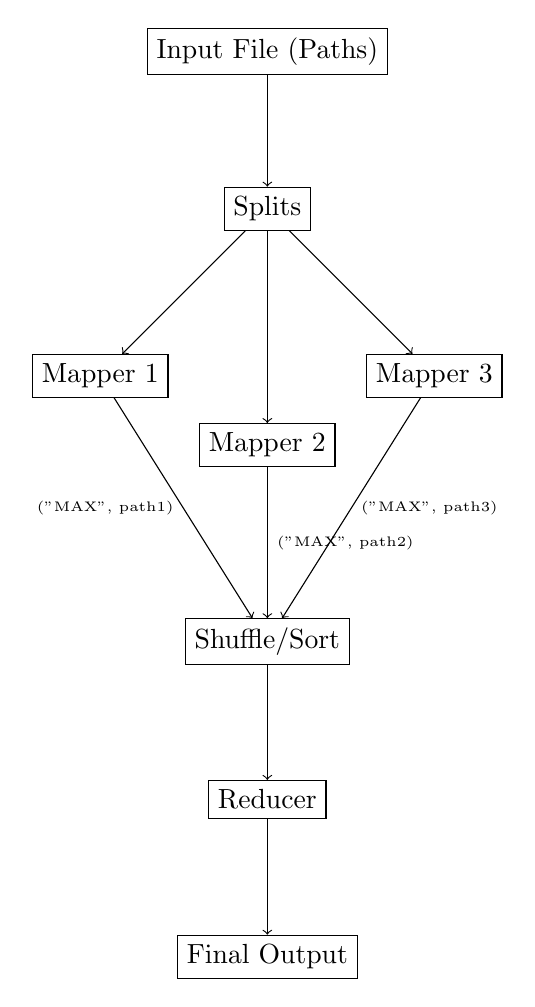
\begin{tikzpicture}[node distance=2cm, auto]
    \node [draw, rectangle] (input) {Input File (Paths)};
    \node [draw, rectangle, below of=input] (split) {Splits};
    
    \node [draw, rectangle, below left of=split, node distance=3cm] (map1) {Mapper 1};
    \node [draw, rectangle, below of=split, node distance=3cm] (map2) {Mapper 2};
    \node [draw, rectangle, below right of=split, node distance=3cm] (map3) {Mapper 3};
    
    \node [draw, rectangle, below of=map2, node distance=2.5cm] (shuffle) {Shuffle/Sort};
    \node [draw, rectangle, below of=shuffle] (reduce) {Reducer};
    \node [draw, rectangle, below of=reduce] (output) {Final Output};

    \draw [->] (input) -- (split);
    \draw [->] (split) -- (map1);
    \draw [->] (split) -- (map2);
    \draw [->] (split) -- (map3);
    
    \draw [->] (map1) -- node[left, font=\tiny] {("MAX", path1)} (shuffle);
    \draw [->] (map2) -- node[font=\tiny] {("MAX", path2)} (shuffle);
    \draw [->] (map3) -- node[right, font=\tiny] {("MAX", path3)} (shuffle);
    
    \draw [->] (shuffle) -- (reduce);
    \draw [->] (reduce) -- (output);
\end{tikzpicture}
\caption{MapReduce Data Flow for Longest Path Problem}
\end{figure}

\section{Implementation}
The system is simulated using Python.

\subsection{Mapper Code}
\begin{lstlisting}[language=Python, caption=Mapper Function]
def mapper(data_chunk):
    local_max_len = 0
    local_max_path = ""
    for path in data_chunk:
        path = path.strip()
        if len(path) > local_max_len:
            local_max_len = len(path)
            local_max_path = path
    return ("MAX", local_max_path)
\end{lstlisting}

\subsection{Reducer Code}
\begin{lstlisting}[language=Python, caption=Reducer Function]
def reducer(mapped_results):
    global_max_len = 0
    global_max_path = ""
    for key, path in mapped_results:
        if len(path) > global_max_len:
            global_max_len = len(path)
            global_max_path = path
    return global_max_path
\end{lstlisting}

\section{Roles and Responsibilities}
\begin{table}[h]
\centering
\begin{tabular}{|c|l|l|}
\hline
\textbf{No.} & \textbf{Member} & \textbf{Task} \\ \hline
1 & Student Name A & Input generation, Mapper implementation \\ \hline
2 & Student Name B & Reducer implementation, Driver code \\ \hline
3 & Student Name C & Report writing, Architecture diagrams \\ \hline
\end{tabular}
\caption{Group Roles}
\end{table}

\end{document}